% #############################################################################
% This is Chapter 5
% !TEX root = ../main.tex
% #############################################################################
% Change the Name of the Chapter i the following line
\fancychapter{Implementation}
\cleardoublepage
% The following line allows to ref this chapter
\label{chapter:implementation}

\noindent To demonstrate our model, we've decided to implement it using a published commercial game, Don't Starve Together and a socially empowered model for agency with proofs given, \ac{FAtiMA} Toolkit.
During this chapter we will explain the inner workings of both Don't Starve Together and \ac{FAtiMA}, and then describe how we managed to implement our model.

In the end of this chapter we will also describe an \ac{NPC} that we published for the Don't Starve Together community, that can be played with.
After reading this chapter, the reader will have the necessary understanding to use our framework to develop an \ac{NPC} for Don't Starve Together.

\section{Don't Starve Together - The Survival Game}

\noindent As described in \ref{chapter:case-study-dst}, Don't Starve Together is a multi-player survival game, in which players either compete or cooperate in order to outlive the opponents and the world.
After reading that section, you will have an understanding of the challenges players face when playing the game.

However, we need to also understand the inner workings of the game.
For the remainder of this section we will explore the game's internal organization in detail, exploring how we can introduce our modifications into the game.

\subsection{Game Modifications}

\noindent In Don't Starve Together, modifications are introduced in the game through the use of the Steam Workshop, a public platform, where players can share modifications for games.
These modifications alter the original content of the game, adding new characters, creating new challenges, but mostly, altering the way the original game works.

In this particular case, the \textit{modders} (the name given to the players who share content on the platform) can alter the content of the game by writing Lua scripts\footnote{Lua is a scripting language and is currently the leading scripting language in games}, which are loaded by the game and modify its content (\href{https://www.lua.org/about.html}{https://www.lua.org/about.html}).
The game itself is already prepared to receive these \textit{mods} (the name given to the modifications published to the platform), and while some kinds of \textit{mods} are somewhat discouraged (like the addition of skins for the games characters), others are encouraged by the developers, who actively support the community in the game's forum.

For a \textit{mod} to be loaded by the game, it has to follow a specific structure and use of a set of helper functions to include the alterations.
As the game content is all written in Lua scripts (which are available to whomever owns a copy of the game)\footnote{The game engine is written in C++, but all the content and functionality is loaded through these Lua scripts}, \textit{modders} are encouraged to check the original game files in order to understand how the game works and how to implement their own changes.

\subsection{Entities}
\label{subsection:entities}

\noindent Everything that exists in the world of Don't Starve Together is represented as an Entity, from the character the player controls, to the sounds the player hears.
These, in turn, are instances of \textit{prefabs} that can be accessed and edited in the Lua scripts used to make the \textit{mods}.
It is important to note that each entity is uniquely identified by a six digit \ac{GUID}.

By specifying and configuring its \textit{components}, \textit{stategraphs}, and \textit{brains}, the \textit{prefabs} define every entity in the game.
Each of these parts represent something different: \textit{components} represent what an entity does; \textit{stategraphs} represent how it looks; and \textit{brains} represent how it behaves.

When a \textit{prefab} is defined, it also configures its \textit{components}, for example, in the definition of the \textit{prefab} ``wood", which contains the \textit{component} ``fuel", there is also the configuration of this \textit{component} that, in comparison to the \textit{prefab} ``charcoal", has a lower level of ``fuel".
Effectively, \textit{components} describe functionalities that a given entity can have, and how that functionality works.
When an entity, either by a player's command or the \textit{brain}'s command, does a chop action, it is the \textit{components} of the held axe that determine how this action will be executed and trigger the appropriate animations and events.

While \textit{components} can be reused throughout different \textit{prefabs} (with different configurations), \textit{brains} are defined on a per \textit{prefab} basis.
Both butterflies and spiders share the ``locomotor" \textit{component}, but have distinct moving behaviours.

When defining the \textit{prefab}, if it is meant to have behaviour, an instance of a \textit{brain} is also defined and attached to the \textit{prefab}.
However, not all \textit{prefabs} have autonomous behaviour, and those that don't, don't have a \textit{brain}.
The \textit{brain} itself is a Behaviour Tree that is attached to an entity, telling it what to do, leaving the part of how to do it up to the entity's \textit{components}.

Using the Lua scripts, a \textit{modder} can create \textit{components}, \textit{stategraphs}, and \textit{brains}.
These can then be attached to existing \textit{prefabs} or new ones, also created by the \textit{modders}.

\section{FAtiMA Toolkit - The AI Agent}

\noindent For the implementation of the \ac{AI} we chose to use \ac{FAtiMA} Toolkit \cite{dias:fatima-modular}, an agent creation toolkit.
As previously discussed in \ref{subsection:fatima}, \ac{FAtiMA} has been successfully used in several social scenarios (\cite{paiva:learning-by-feeling} \cite{rodrigues:i-can-feel-to} \cite{aylett:intercultural-empathy} \cite{correia:sueca}), making it the best choice for our implementation.

In this section, we present the Authoring Tools available to work with the toolkit.
Throughout this section, we will use the term developer to refer to someone who uses the FAtiMA-Toolkit to create agents.

\subsection{The Authoring Tools}

\begin{figure}
  \centering
  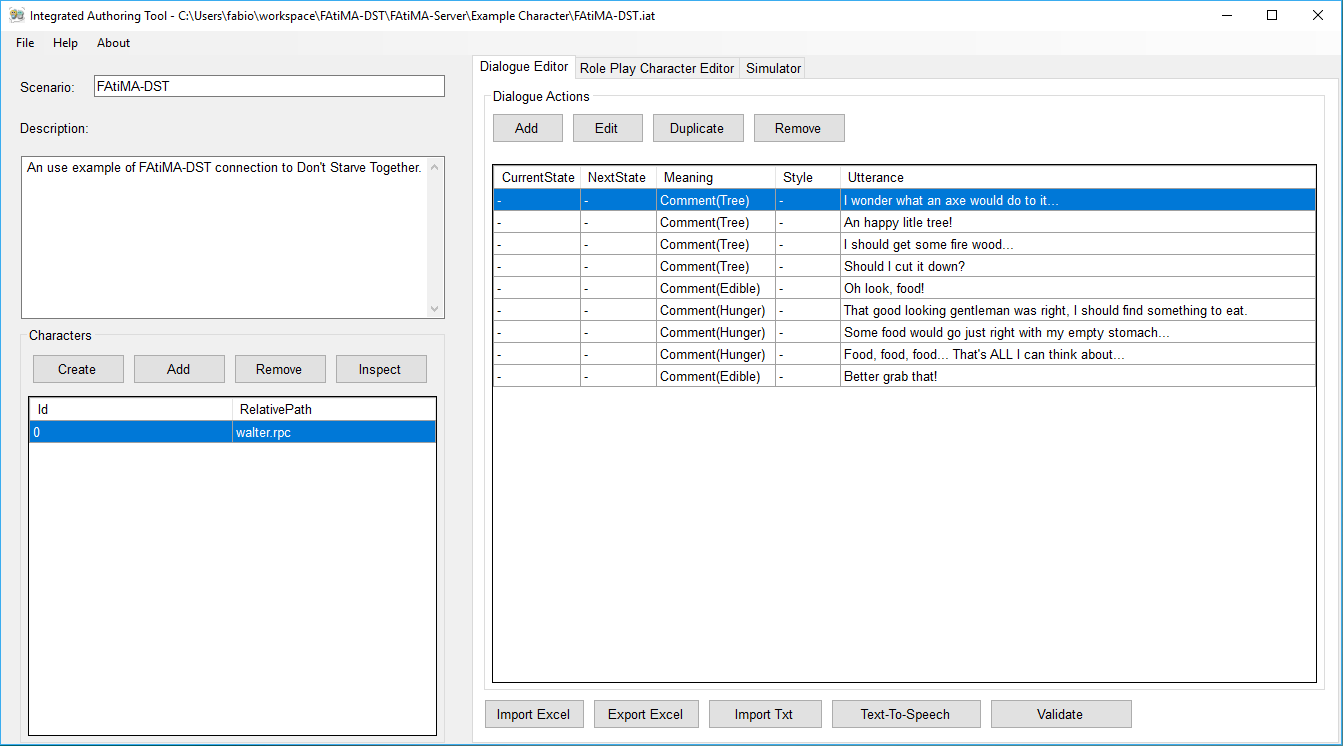
\includegraphics[width=\textwidth]{./Images/iat-interface}
  \caption{The Integrated Authoring Tool for \ac{FAtiMA} Toolkit.}
  \label{fig:iat-interface}
\end{figure}

\noindent The easiest way to develop a character with \ac{FAtiMA} Toolkit is by using the provided Authoring Tools.
Every implemented asset (described in \ref{subsection:fatima}) comes with a \ac{GUI} Tool which provides facilities to help develop a character.

The main tool is the \ac{IAT}, which can be seen in Figure \ref{fig:iat-interface}.
Through the \ac{IAT}, developers can access every other asset to develop their agents.
Developers can create dialogues, \acp{RPC} (and its components: Emotional Decision Making, Emotional Appraisal, etc.), run a chat simulator, and simulate and inspect \acp{RPC}.

In Figure \ref{fig:iat-interface} a set of dialogues from the example provided with our platform, Walter, can be seen.
The developer can use the example provided to create her own \acp{RPC}, and then use the Authoring Tools to test them.
The \ac{RPC} Inspector gives developers the possibility to provide a set of events that will be perceived by the \ac{RPC}.
The developer can then execute the contained scenario to see the emotional appraisal and decision processes in action.

\section{Putting it together}

\noindent Now that we have explored both the game used as a scenario and the technology used to control the characters, its time to look at how we connected both.
For the rest of this section, we'll present the implementation of the framework, explaining in full detail the decisions made.

The implementation itself consists in two modules: FAtiMA-DST, a Don't Starve Together \textit{mod}; and FAtiMA-Server, a C\# console application.
Both these modules have been made publicly available on the Github repository \href{https://github.com/hineios/FAtiMA-DST}{https://github.com/hineios/FAtiMA-DST}.
In the repository there is also a guide to help anyone develop an \ac{NPC} for Don't Starve Together.
As shown in Figure \ref{fig:implementation}, the communication between the two modules is made using \ac{HTTP}, which transfers \ac{JSON} objects back and forth.

The choice of using \ac{HTTP} communication arouse from a limitation we found while developing the initial proof of concept for this implementation.
Initially, we considered importing the \ac{FAtiMA} Toolkit directly, as the loading of C\# \ac{DLL} files into a Lua interpreter is possible.
However, as a security measure, the Lua interpreter embedded in \ac{DST} blocks any importation of external libraries.
The inclusion of malicious libraries through the Steam Workshop would be a major security issue for both the company and the players.

As alternatives, we considered using textual files or a relational database that would act as a proxy between the modules, but we finally decided to use an \ac{HTTP} connection as the game provided an easy way to make requests and register callback functions to handle the responses.
Due to the client-server nature of \ac{HTTP} however, the FAtiMA-DST module continuously makes \ac{HTTP} requests with \ac{JSON} encoded data to the FAtiMA-Server module, which handles these requests yielding an appropriate response (also \ac{JSON} encoded).
As a data-interchange format, \ac{JSON} provides the necessary abstraction to exchange information between C\# objects and Lua tables.

\begin{figure}
  \centering
  
\includegraphics[width=\textwidth]{./Images/implementation}
  \caption{A graphical representation of the implementation.}
  \label{fig:implementation}
\end{figure}

\subsection{FAtiMA-Server}

\noindent The FAtiMA Toolkit is written in C\# and published as a set of DLL libraries.
Taking this into account, we decided to implement a simple server in C\#, capable of handling the \ac{HTTP} requests made by FAtiMA-DST \textit{mod}.
This server contains a list of Role Play Character Assets that are uniquely linked with the agents running on the scenario.
Each request the server handles has an entity's (\ac{NPC}) \ac{GUID}, which is used to also identify a Role Play Character Asset.

Additionally, requests are divided into three categories: perceptions, events, and decisions.
Perception requests contain information on the \ac{NPC}'s state and field of vision, and happen periodically.
Event requests contain information on relevant world events, and happen whenever an event is triggered.
Decision requests trigger the decision process that tells the \ac{NPC} what to do, and happen periodically.

If we consider the flow of information, the first two types (perception and event requests) represent a flow of information from the embodiment to the \ac{AI}, while the third (decision requests) represents a flow of information from the \ac{AI} to the embodiment.

When received, perception requests are translated into a series of Property-Changed events, that update the \ac{RPC}'s Knowledge Base.
Event requests will be translated to Action-End events and decision requests will trigger the \ac{RPC}'s decision process for the appropriate layer.

It is important to notice the limitations of using \ac{HTTP} as the method of communication.
This form of communication makes it impossible for the \ac{AI} to give direct actions to the embodiment, as we cannot send messages from the server to the client, only respond to client's requests.
As such, we have to rely on periodic requests made by the embodiment that will cause the \ac{AI} to make a decision and respond with an action.

\subsection{FAtiMA-DST}

\noindent This module was implemented as a \textit{brain} for \ac{DST} and is responsible to send perceptions to FAtiMA-Server and execute the actions it returns.
To achieve this, it sends a perception request to FAtiMA-Server two times a second, a decision request for behaviour every one and a half second, and a decision request for dialogue every ten seconds.
The values were tested and tweaked for the best compromise between behaviour and performance.

To send the perceptions to the FAtiMA-Server, it counts with a set of helper functions that extract the necessary information from surrounding entities.
A set of listeners relay information about events to the FAtiMA-Server, and a Behaviour Tree executes actions received from the FAtiMA-Server.
For a complete list of beliefs check Tables \ref{tab:state-beliefs} and \ref{tab:world-state-beliefs} and for actions refer to the Appendix \ref{appendix:A}

The Behaviour Tree makes use of the built-in Buffered Actions to execute the actions.
This provides a layer of abstraction over actions to handle all the locomotion details and appropriate verifications (e.g. it is only possible to chop a tree if an axe is held).

To handle the FAtiMA-Server commands, the tree contains two nodes: a node that executes actions (via buffered actions), and a node that handles the special behaviour of wandering.
The handling of dialogue is independent from the behaviour and is executed immediately without making use of the behaviour tree.

\section{Creating Walter}

\noindent As an example \ac{NPC}, we've implemented a model based agent to demonstrate how one could use the set of available beliefs to create behaviour.
This example only makes use of FAtiMA's Dialogue Manager and Emotional Decision Making assets.
%Using the provided examples from the toolkit and this example, developers will be able to create more complex \ac{NPC}s by making use of these and other assets.

This example has been published to the Steam Workshop in the form of an \ac{AI} companion, an \ac{NPC} named Walter \footnote{The \textit{mod} public page can be found in this link: \href{http://steamcommunity.com/sharedfiles/filedetails/?id=1339264854}{http://steamcommunity.com/sharedfiles/filedetails/?id=1339264854}}.
On the \textit{mod}'s public page, a set of instructions can be found on how to run the character.
The page also contains links to the public repository where all the code for this framework can be found.

% For the remainder of this section we will describe in detail the currently available beliefs and actions and how can these be used to create a \ac{NPC} using Walter as an example.

% \subsection{Beliefs}

The current set of beliefs available can be divided into two groups: character's state beliefs and world's state beliefs.
The complete listing of the beliefs is presented in tables \ref{tab:state-beliefs} and \ref{tab:world-state-beliefs}.
Most of them are self explanatory, but others require some explanation.

\begin{table}[htb]
	\centering
    \caption{Character's state beliefs}
    \label{tab:state-beliefs}
    \begin{tabular}{ | p{0.35\linewidth} | p{0.6\linewidth} | }
        \hline 
        \textbf{Belief} & \textbf{Description} \\ \hline \hline
        \texttt{Health([name]) = [value]} & Describes the agent's (\textit{name}) health \\ \hline
        \texttt{Hunger([name]) = [value]} & Describes the agent's (\textit{name}) hunger \\ \hline
        \texttt{Sanity([name]) = [value]} & Describes the agent's (\textit{name}) sanity \\ \hline
        \texttt{Moisture([name]) = [value]} & Describes the agent's (\textit{name}) moisture level \\ \hline
        \texttt{Temperature([name]) = [value]} & Describes the agent's (\textit{name}) temperature \\ \hline
        \texttt{IsFreezing([name]) = [bool]} & Describes if the agent (\textit{name}) is taking damage from extreme cold \\ \hline
        \texttt{IsOverheating([name]) = [bool]} & Describes if the agent (\textit{name}) is taking damage from extreme hot \\ \hline
        \texttt{IsBusy([name]) = [bool]} & Describes if the agent (\textit{name}) is currently executing any action \\ \hline
        \texttt{PosX([name]) = [value]} & The agent's (\textit{name}) current X position \\ \hline
        \texttt{PosZ([name]) = [value]} & The agent's (\textit{name}) current Z position \\ \hline
        \texttt{InLight([name]) = [bool]} & Defines if the agent (\textit{name}) is in the light or darkness \\ \hline
        \texttt{InSight([GUID]) = [bool]} & What the agent (\textit{name}) is currently seeing \\ \hline
        \texttt{InInventory([GUID]) = [bool]} & What the agent (\textit{name}) has in his inventory \\ \hline
        \texttt{IsEquipped([GUID]) = [bool]} & What the agent (\textit{name}) has equipped \\ \hline
    \end{tabular}
\end{table}

\begin{figure}
  \centering
  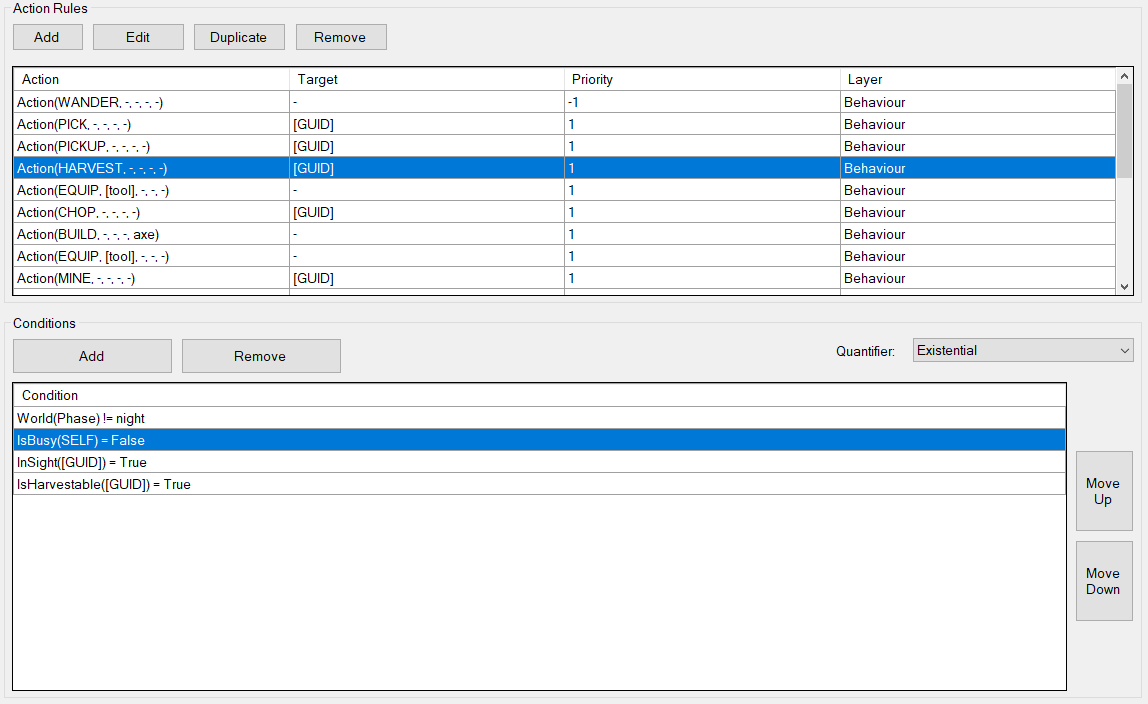
\includegraphics[width=\textwidth]{./Images/isbusy-example}
  \caption{Walter's \texttt{HARVEST} action.}
  \label{fig:harvest-example}
\end{figure}

The \texttt{IsBusy} belief is used to represent if the \ac{NPC} is executing an action.
As the implementation stands, if an action is received by FAtiMA-DST, the \ac{NPC} will immediately execute that action.
This allows for reactive behaviour and prevents the overlap of actions with equal priority.

The developer should use this belief as a condition for actions, as shown in Figure \ref{fig:harvest-example}, and omit this condition for actions that should be executed even if another one is being executed, as shown in Figure \ref{fig:equiptorch-example}.
In this example, equipping the torch can overlap other actions as it represents a case of life and death for the \ac{NPC} (being in the dark will get the \ac{NPC} dead).

\begin{figure}
  \centering
  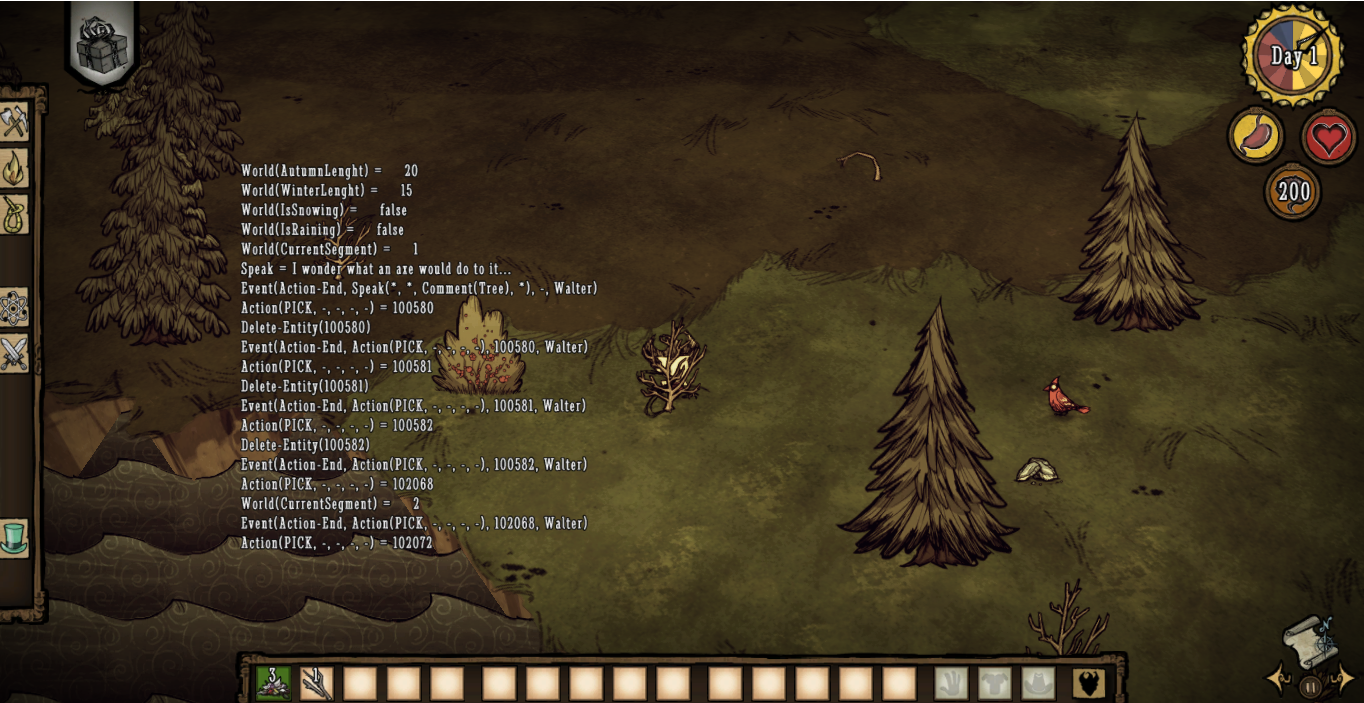
\includegraphics[width=\textwidth]{./Images/action-example-with-debug}
  \caption{Walter executing a \texttt{PICK} action with debug information being displayed in an overlay.}
  \label{fig:action-example-with-debug}
\end{figure}

\texttt{InLight}, \texttt{InSight}, and \texttt{InInventory} are in fact beliefs about entities.
However, they are presented here as they represent the state of entities in relation to the \ac{NPC}.
For example, Walter will only try to harvest any given entity if it is in sight, as shown in Figure \ref{fig:harvest-example}.
The use of these three beliefs is highly recommended when the action requires interaction of the \ac{NPC} with other entities.
The \ac{NPC} should not try to directly pick or pick up entities that she cannot see as they may no longer exist.

Do note that most of these beliefs require the agent's name.
While defining the Decision Making Asset rules, the special keyword \texttt{SELF} should be used for this purpose.
In Figure \ref{fig:action-example-with-debug} we can see the \ac{NPC} executing an action with some debug information being displayed in an overlay.

\begin{figure}
  \centering
  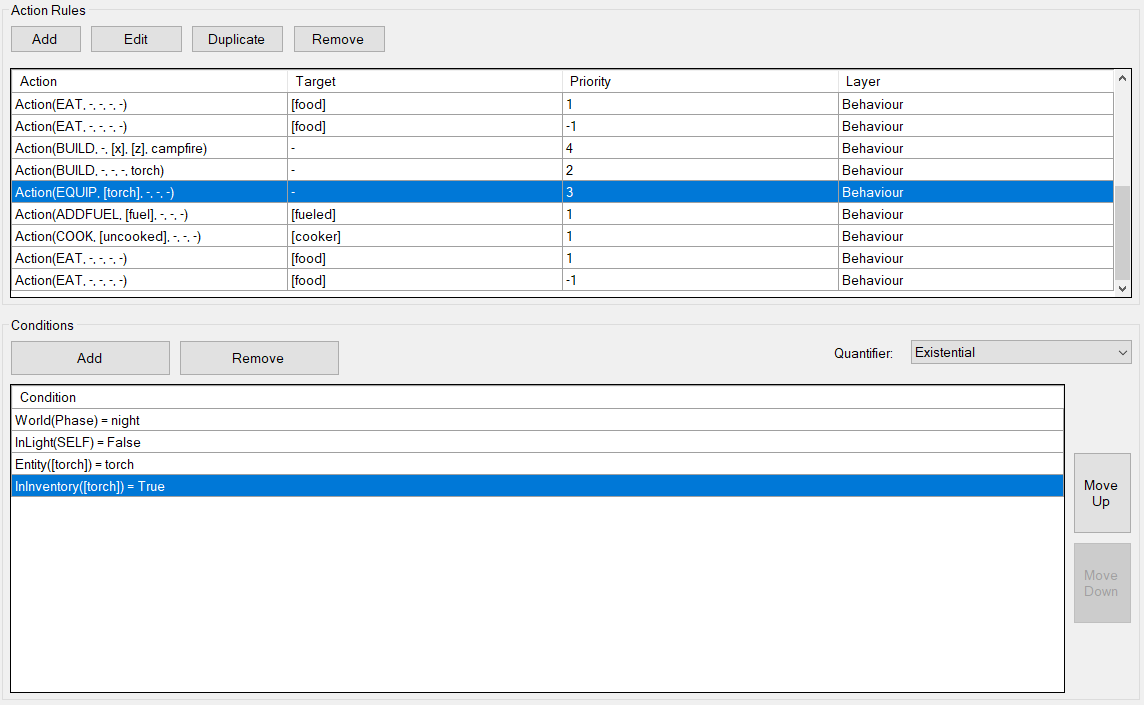
\includegraphics[width=\textwidth]{./Images/ininventory-example}
  \caption{Walter's \texttt{EQUIP} torch example.}
  \label{fig:equiptorch-example}
\end{figure}

\begin{table}[htb]
	\centering
    \caption{World's State beliefs}
    \label{tab:world-state-beliefs}
    \begin{tabular}{ | p{0.35\linewidth} | p{0.6\linewidth} | }
        \hline 
        \textbf{Belief} & \textbf{Description} \\ \hline \hline
        \texttt{Entity([GUID]) = [prefab]} & Defines an entity \\ \hline 
        \texttt{Quantity([GUID]) = [quantity]} & Defines how big is the stack (\textit{quantity}) of a given entity \\ \hline 
        \texttt{IsCollectable([GUID]) = [bool]} & True if the given entity is pickable (collect natural resources). \textit{PICK} action \\ \hline 
        \texttt{IsCooker([GUID]) = [bool]} & True if the given entity can cook other entities. \textit{COOK} action \\ \hline 
        \texttt{IsCookable([GUID]) = [bool]} & True if the given entity can be cooked. \textit{COOK} action \\ \hline 
        \texttt{IsEdible([GUID]) = [true]} & True if the entity may be eaten by the curent character (it takes into account the character's diet). \textit{EAT} action \\ \hline 
        \texttt{IsEquippable([GUID]) = [bool]} & True if the given entity may be equipped. \textit{EQUIP} action \\ \hline 
        \texttt{IsFuel([GUID]) = [bool]} & True if the given entity may be used to fuel stuff. \textit{FUEL} action \\ \hline 
        \texttt{IsFueled([GUID]) = [bool]} & True if the given entity requires fuel to function. \textit{FUEL} action \\ \hline 
        \texttt{IsGrower([GUID]) = [bool]} & True if the given entity can be used to grow seeds. \textit{PLANT} action \\ \hline 
        \texttt{IsHarvestable([GUID]) = [bool]} & True if the given entity is ready to be harvested. \textit{HARVEST} action \\ \hline 
        \texttt{IsPickable([GUID]) = [bool]} & True if the given entity is pickable (pick stuff from the ground). \textit{PICKUP} action \\ \hline 
        \texttt{IsStewer([GUID])= [bool]} & True if the given entity can take other entities to cook recipes \\ \hline 
        \texttt{IsChoppable([GUID]) = [bool]} & True if the given entity is workable by an axe. \textit{CHOP} action \\ \hline 
        \texttt{IsDiggable([GUID]) = [bool]} & True if the given entity is workable by a shovel. \textit{DIG} action \\ \hline 
        \texttt{IsHammerable([GUID]) = [bool]} & True if the given entity is workable by a hammer. \textit{HAMMER} action \\ \hline 
        \texttt{IsMineable([GUID]) = [bool]} & True if the given entity is workable by a pick. \textit{MINE} action \\ \hline 
        \texttt{PosX([GUID]) = [value]} & Defines the X coordinate (\textit{value}) of an entity \\ \hline 
        \texttt{PosZ([GUID]) = [value]} & Defines the Z coordinate (\textit{value}) of an entity \\ \hline 
        \texttt{World(CurrentSegment) = [value]} & The current segment, ranges between 0 and 15 \\ \hline 
        \texttt{World(Cycle) = [value]} & Defines how many cycles (days) have passed since the start of the game \\ \hline 
        \texttt{World(Phase) = [value]} & Defines the phase of the day. \textit{value} can be: 'day', 'dusk', or 'night' \\ \hline 
        \texttt{World(PhaseLenght, [phase]) = [value]} & The current duration of the day \textit{phase} in clock segments. The sum of all segments is always 16 \\ \hline 
        \texttt{World(Season) = [value]} & Defines the current season. \textit{value} can be: 'spring', 'summer', 'autumn', or 'winter' \\ \hline 
        \texttt{World(SeasonProgress) = [value]} & A value between 0 and 1 that defines the progress of the season \\ \hline 
        \texttt{World(ElapsedDaysInSeason) = [value]} & How many days have passed in the current season \\ \hline 
        \texttt{World(RemainingDaysInSeason) = [value]} & How many days are left to the end of the season \\ \hline 
        \texttt{World(SpringLength) = [value]} & Defines the current lenght of Spring \\ \hline 
        \texttt{World(SummerLength) = [value]} & Defines the current lenght of Summer \\ \hline 
        \texttt{World(AutumnLenght) = [value]} & Defines the current lenght of Autumn \\ \hline 
        \texttt{World(WinterLenght) = [value]} & Defines the current lenght of Winter \\ \hline 
        \texttt{World(IsSnowing) = [bool]} & True if it is snowing \\ \hline 
        \texttt{World(IsRaining) = [bool]} & True if it is raining \\ \hline 
        \texttt{World(MoonPhase) = [value]} & Defines the current moon phase. \textit{value} can be: 'new', 'quarter', 'half', 'threequarter', or 'full' \\ \hline 
	\end{tabular}
\end{table}

As far as world state beliefs go (described in Table \ref{tab:world-state-beliefs}), these are used to represent both the state of the world and entities present in the world.

Most beliefs used to describe entities coincide with the presence of certain \textit{components} (as described in \ref{subsection:entities}).
The use of these beliefs as conditions for the appropriate actions is highly encouraged as they will prevent the \ac{NPC} from trying to execute actions she cannot execute.

Walter will only harvest resources if the \texttt{IsHarvestable} belief is true, as depicted in Figure \ref{fig:harvest-example}.
This is also true for every other action present in Walter's decision rules.

Despite this, one can use the prefab of an entity as a condition, such as Walter does when equipping a torch (Figure \ref{fig:equiptorch-example}).
This will allow the creation of more refined behaviour.

Appendix \ref{appendix:A} contains two tables which have a comprehensive list of all available actions, Tables \ref{tab:actions-1} and \ref{tab:actions-2}.
Both tables also contain a brief description of every action, which along side the existing example of Walter, will help developers write their own behaviour rules.

\subsection{Dialogue}

\noindent As far as speech goes, the current framework has some limitations.
Currently, there is no two-way communication, meaning that, although the agent can speak (through the use of text), the players will not be able to respond.
In Figure \ref{fig:axe-dialogue} we can see the execution of a speak action by the agent while he is executing another action.

\begin{figure}
  \centering
  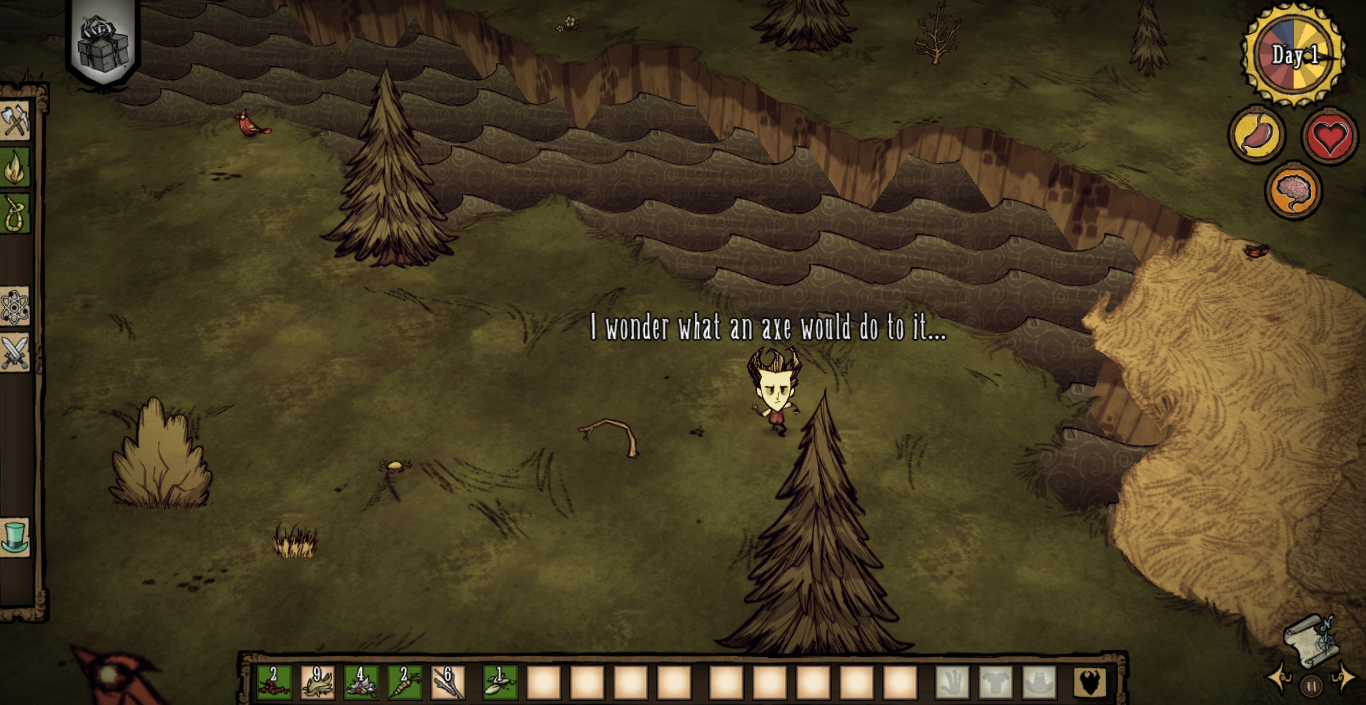
\includegraphics[width=\textwidth]{./Images/axe-dialogue}
  \caption{Example of speak action.}
  \label{fig:axe-dialogue}
\end{figure}

\begin{figure}
  \centering
  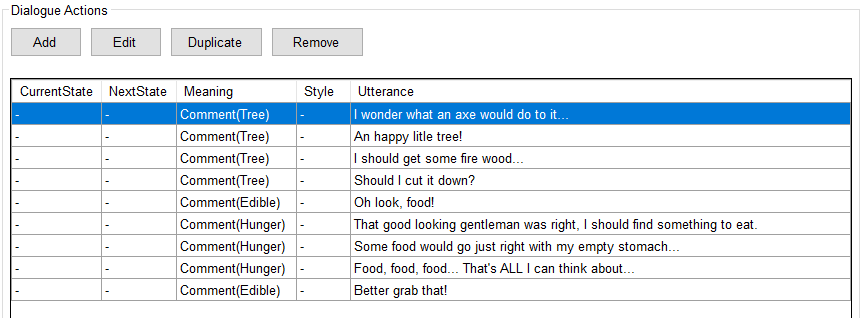
\includegraphics[width=\textwidth]{./Images/dialogue-example}
  \caption{Walter's available dialogues.}
  \label{fig:dialogue-example}
\end{figure}

To make an \ac{NPC} speak, the developer will need to create the available utterances using the Dialogue Editor as depicted in Figure \ref{fig:dialogue-example}.
Multiple utterances can be created with the same meaning, allowing for variety in the \ac{NPC}'s dialogue.
In Walter's example, several utterances have been added for each meaning.

To trigger these sentences, the developer also needs to add a rule with the appropriate layer to the decision making asset, as shown in Figure \ref{fig:dialogue-action-example}.
Here we can see, that in order for Walter to say a comment about hunger, his \texttt{Hunger} belief has to have a value lower than seventy.

\begin{figure}
  \centering
  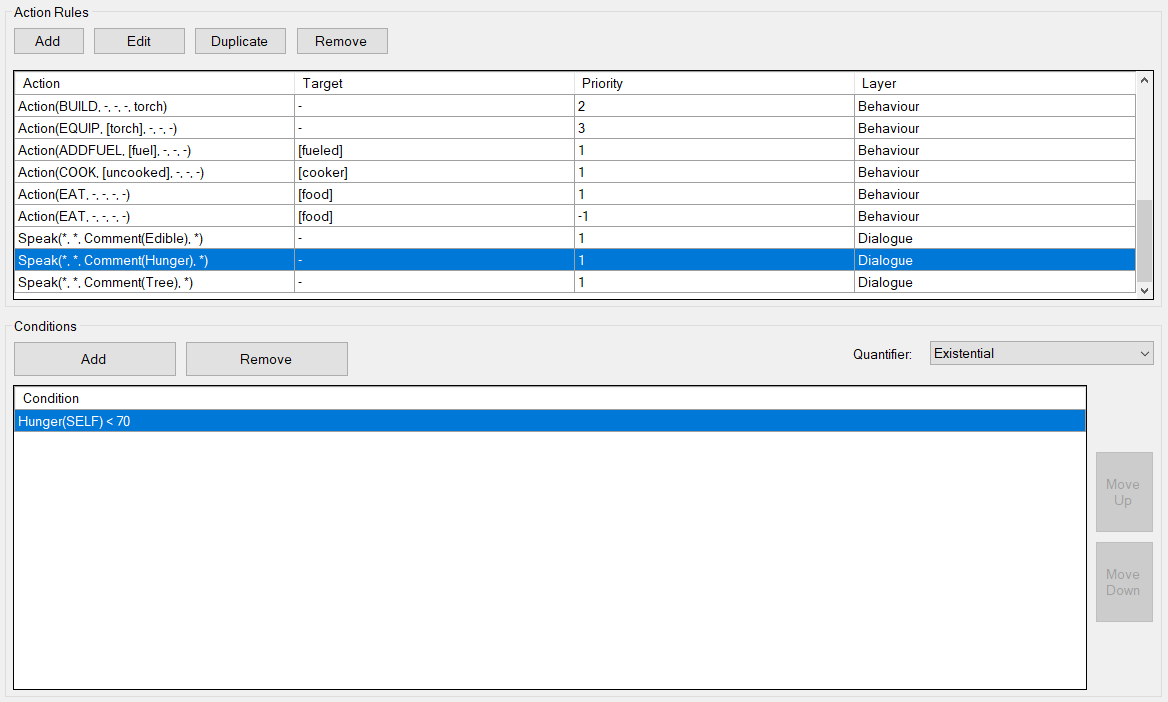
\includegraphics[width=\textwidth]{./Images/dialogue-action-example}
  \caption{Walter's dialogue action rule.}
  \label{fig:dialogue-action-example}
\end{figure}

The addition of these sentences allows players to better understand the \ac{NPC}'s decision process.
By stating some random utterances about its current state, we can transmit the characters state of mind to the players.
These sentences can also be used to transmit the \ac{NPC} emotional state, needs, and goals.

\section{Playing with Walter}

\begin{figure}
  \centering
  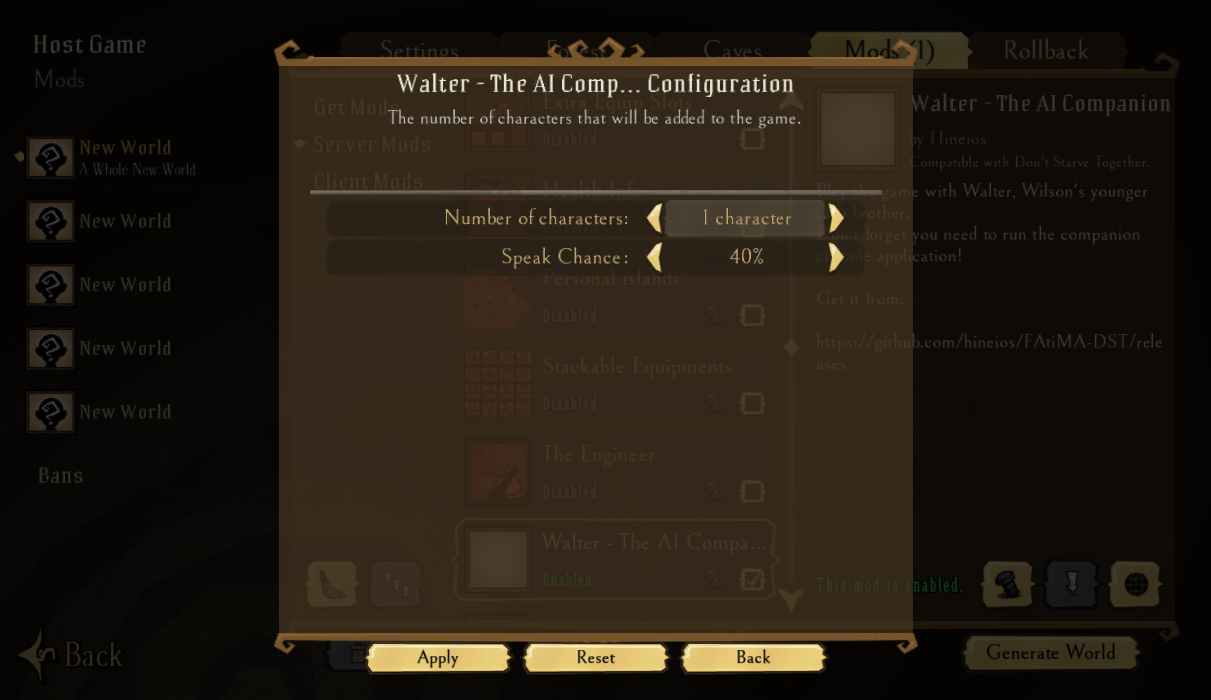
\includegraphics[width=\textwidth]{./Images/mod-config}
  \caption{Configuration screen for FAtiMA-DST.}
  \label{fig:mod-config}
\end{figure}

In order to run our framework, players will have to run FAtiMA-Server by launching the console application available at the public repository.
FAtiMA-Server will automatically listen to \ac{HTTP} requests on port 8080.
Then, before launching a game, the player will need to activate and configure the \textit{mod} as shown in Figure \ref{fig:mod-config}.
When the game is launched, the number of characters specified will spawn in the same place that players spawn.

\begin{figure}
  \centering
  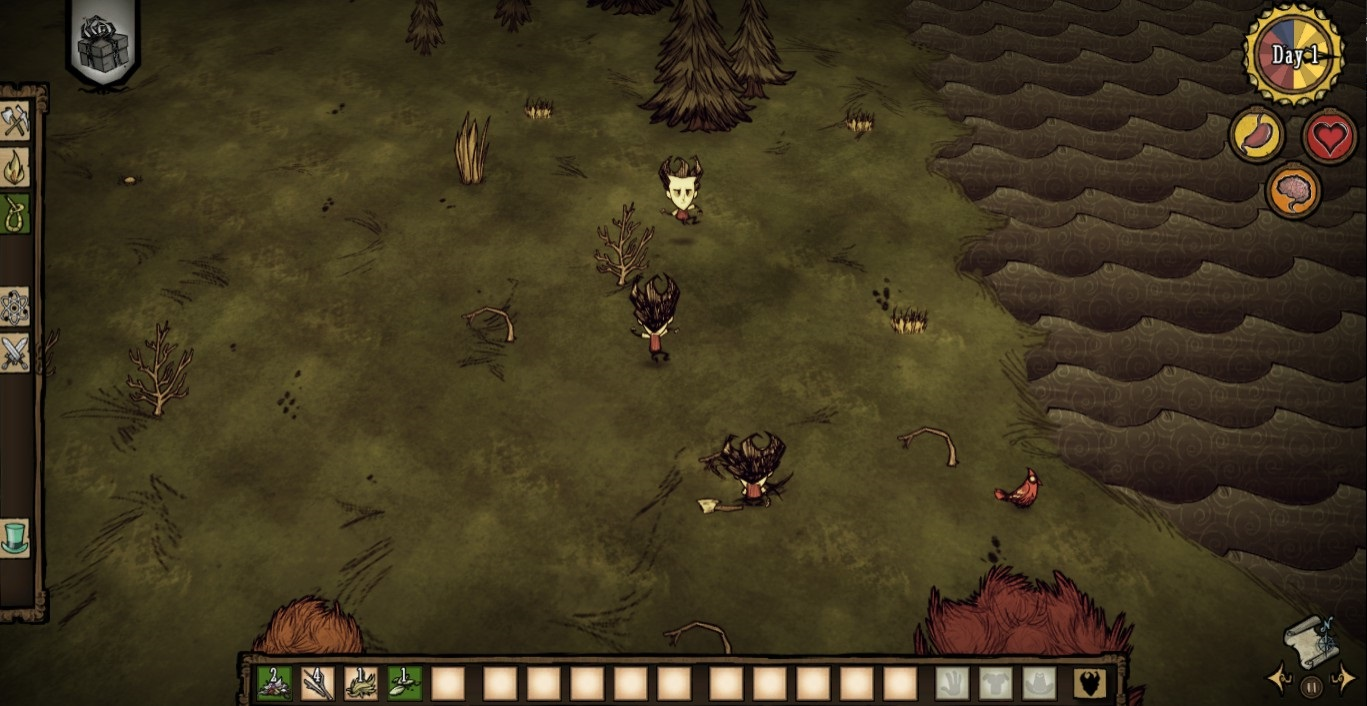
\includegraphics[width=\textwidth]{./Images/multiple-agents}
  \caption{A player (center) playing the \textit{mod} with two FAtiMA controlled characters (top and bottom).}
  \label{fig:multiple-agents}
\end{figure}

In Figure \ref{fig:multiple-agents}, we can see an example of a player playing the game with two \acp{NPC} being controlled by \ac{FAtiMA}.
